\section{Differential Corrections}\label{sec:DifferentialCorrections}
Differential corrections are employed to compute solutions in targeting problems that satisfy the
provided constraints on the initial condition and the trajectory arc. To do so, it is necessary to
relate constraints on the trajectory to any parameters in the problem that are free to vary through
Jacobians such as the state transition matrix. In this investigation, the targeting process is
accomplished via multi-variable Newton-Raphson methods.

\subsection{State Transition Matrix}
The state transition matrix (STM) relates variations in an initial state, $\qbar_{0}=\qbar(t_{0})$,
to variations in a downstream state $\qbar(t)$. Starting from a first-order Taylor series expansion
about the baseline trajectory arc, the linear variational equation is derived:
\begin{equation}
    \partial\qbardot(t)=A(t)\partial\qbar(t),
    \label{eq:linearvariational}
\end{equation}
where $A(t)$ is the Jacobian matrix for the equations of motion with respect to the state at time
$t$. A full derivation for the CR3BP $A(t)$ matrix is found in Zimovan, but the result is given
here\cite{Zimovan:2017}:
\vfill
\begin{equation}
    A(t)=\begin{bmatrix}    \frac{\partial x}{\partial x_{0}}       &   \frac{\partial x}{\partial y_{0}}       &   \frac{\partial x}{\partial z_{0}}       &   \frac{\partial x}{\partial \xdot_{0}}       &   \frac{\partial x}{\partial \ydot_{0}}       &   \frac{\partial x}{\partial \zdot_{0}}       \\
                            \frac{\partial y}{\partial x_{0}}       &   \frac{\partial y}{\partial y_{0}}       &   \frac{\partial y}{\partial z_{0}}       &   \frac{\partial y}{\partial \xdot_{0}}       &   \frac{\partial y}{\partial \ydot_{0}}       &   \frac{\partial y}{\partial \zdot_{0}}       \\
                            \frac{\partial z}{\partial x_{0}}       &   \frac{\partial z}{\partial y_{0}}       &   \frac{\partial z}{\partial z_{0}}       &   \frac{\partial z}{\partial \xdot_{0}}       &   \frac{\partial z}{\partial \ydot_{0}}       &   \frac{\partial z}{\partial \zdot_{0}}       \\
                            \frac{\partial \xdot}{\partial x_{0}}   &   \frac{\partial \xdot}{\partial y_{0}}   &   \frac{\partial \xdot}{\partial z_{0}}   &   \frac{\partial \xdot}{\partial \xdot_{0}}   &   \frac{\partial \xdot}{\partial \ydot_{0}}   &   \frac{\partial \xdot}{\partial \zdot_{0}}   \\
                            \frac{\partial \ydot}{\partial x_{0}}   &   \frac{\partial \ydot}{\partial y_{0}}   &   \frac{\partial \ydot}{\partial z_{0}}   &   \frac{\partial \ydot}{\partial \xdot_{0}}   &   \frac{\partial \ydot}{\partial \ydot_{0}}   &   \frac{\partial \ydot}{\partial \zdot_{0}}   \\
                            \frac{\partial \zdot}{\partial x_{0}}   &   \frac{\partial \zdot}{\partial y_{0}}   &   \frac{\partial \zdot}{\partial z_{0}}   &   \frac{\partial \zdot}{\partial \xdot_{0}}   &   \frac{\partial \zdot}{\partial \ydot_{0}}   &   \frac{\partial \zdot}{\partial \zdot_{0}}   \end{bmatrix}
        =\begin{bmatrix}    0                                       &   0                                       &   0                                       &   1   &   0   &   0   \\
                            0                                       &   0                                       &   0                                       &   0   &   1   &   0   \\
                            0                                       &   0                                       &   0                                       &   0   &   0   &   1   \\
                            \frac{\partial U}{\partial x\partial x} &   \frac{\partial U}{\partial x\partial y} &   \frac{\partial U}{\partial x\partial z} &   0   &   2n  &   0   \\
                            \frac{\partial U}{\partial y\partial x} &   \frac{\partial U}{\partial y\partial y} &   \frac{\partial U}{\partial y\partial z} &   -2n &   0   &   0   \\
                            \frac{\partial U}{\partial z\partial x} &   \frac{\partial U}{\partial z\partial y} &   \frac{\partial U}{\partial z\partial z} &   0   &   0   &   0   \end{bmatrix},
                            \label{eq:variationalJacobian}
\end{equation}
\vspace{1mm}
\begin{equation}
    \frac{\partial U}{\partial x\partial x}=1-\frac{1-\mu}{d^{3}}-\frac{\mu}{r^{3}}+\frac{3(1-\mu)(x+\mu)^{2}}{d^{5}}+\frac{3\mu(x-1+\mu)^{2}}{r^{5}},
    \label{eq:partialUpartialxx}
\end{equation}
\vspace{1mm}
\begin{equation}
    \frac{\partial U}{\partial x\partial y}=\frac{\partial U}{\partial y\partial x}=\frac{3(1-\mu)(x+\mu)y}{d^{5}}+\frac{3\mu(x-1+\mu)y}{r^{5}},
    \label{eq:partialUpartialxy}
\end{equation}
\vspace{1mm}
\begin{equation}
    \frac{\partial U}{\partial x\partial z}=\frac{\partial U}{\partial z\partial x}=\frac{3(1-\,u)(x+\mu)z}{d^{5}}+\frac{3\mu(x-1+\mu)z}{r^{5}},
    \label{eq:partialUpartialxz}
\end{equation}
\vspace{1mm}
\begin{equation}
    \frac{\partial U}{\partial y\partial y}=1-\frac{1-\mu}{d^{3}}-\frac{\mu}{r^{3}}+\frac{3(1-\mu)y^{2}}{d^{5}}+\frac{3\mu y^{2}}{r^{5}},
    \label{eq:partialUpartialyy}
\end{equation}
\vspace{1mm}
\begin{equation}
    \frac{\partial U}{\partial y\partial z}=\frac{\partial U}{\partial z\partial y}=\frac{3(1-\mu)yz}{d^{5}}+\frac{3\mu yz}{r^{5}},
    \label{eq:partialUpartialyz}
\end{equation}
\vspace{1mm}
\begin{equation}
    \frac{\partial U}{\partial z\partial z}=-\frac{1-\mu}{d^{3}}-\frac{\mu}{r^{3}}+\frac{3(1-\mu)z^{2}}{d^{5}}+\frac{3\mu z^{2}}{r^{5}}.
    \label{eq:partialUpartialzz}
\end{equation}
The solution to \cref{eq:linearvariational}:
\begin{equation}
    \partial\qbar(t)=\frac{\partial\qbar(t)}{\partial\qbar_{0}}\partial\qbar_{0},
    \label{eq:variationalsolution}
\end{equation}
is rearranged to provide the STM $\Phi(t,t_{0})$:
\begin{equation}
    \Phi(t,t_{0})=\frac{\partial\qbar(t)}{\partial\qbar_{{0}}}.
    \label{eq:STM}
\end{equation}
The equation for the STM is appended to the CR3BP equations of motion when propagating:
\begin{equation}
    \dot{\Phi}(t,t_{0})=A(t)\Phi(t,t_{0}),
    \label{eq:STMEoM}
\end{equation}
where the initial condition is $\Phi(t_{0},t_{0})=I_{6\times6}$.

\subsection{Multi-Variable Newton-Raphson Method}
Targeting problems require iterative approaches where an initial guess is updated until it meets a
set of constraints to solve a boundary value problem. This investigation employs a multi-variable
Newton-Raphson method as a differential corrections process for single-shooting targeting problems,
applying analytical or numerical partial derivatives of constraints with respect to the initial
conditions. The Newton-Raphson iterative approach facilitates convergence to local solutions that
satisfy the boundary conditions.

If $\Xbar$ is a free variable vector and $\Fbar(\Xbar)$ is a constraint vector that is dependent on
the free variables, then the goal of the targeting problem is to find $\Xbar$ such that
$\Fbar(\Xbar)=\zerobar$ (to a selected tolerance). Example free variable and constraint vectors
are introduced in future sections. Applying the Newton-Raphson method, the update equation is
provided by a first-order Taylor series expansion about the initial condition $\Xbar_{0}$:
\begin{equation}
    \Fbar(\Xbar)=\Fbar(\Xbar_{0})+DF(\Xbar_{0})(\Xbar-\Xbar_{0})=\zerobar,
    \label{eq:updateequation}
\end{equation}
where $DF(\Xbar)$ is the Jacobian containing the partial derivatives of the constraints with
respect to the free variables. With the update equation, the next iteration on the initial
conditions is computed. If the number of free variables matches that of the constraints:
\begin{equation}
    \Xbar=\Xbar_{0}-DF(\Xbar_{0})^{-1}\Fbar(\Xbar_{0}),
    \label{eq:NRsolution}
\end{equation}
and $\Xbar$ becomes the new iteration of the initial conditions. Ideally, upon each iteration, the
norm of the constraint vector approaches closer to the tolerance. If the number of free variables
is greater than the number of constraints, a minimum-norm solution is computed:
\begin{equation}
    \Xbar=\Xbar_{0}-DF(\Xbar_{0})^{T}(DF(\Xbar_{0})DF(\Xbar_{0})^{T})^{-1}\Fbar(\Xbar_{0}).
    \label{eq:minimumnorm}
\end{equation}
When the number of free variables is less than the number of constraints, a least squares solution
is employed, but that is not addressed in this investigation.

As a simple targeting example, consider the following planar boundary value problem in
\cref{fig:targeting}. The objective is to vary the initial velocity and time-of-flight (TOF) to
target a desired final position $\rhobar_{d}$. This results in a free variable vector:
\begin{equation}
    \Xbar=\begin{bmatrix}   \xdot_{0}   &   \ydot_{0}   &   \tau    \end{bmatrix}^{T},
    \label{eq:exfreevar}
\end{equation}
and constraint vector:
\begin{equation}
    \Fbar(\Xbar)=\begin{bmatrix}    x_{f}-x_{d} &   y_{f}-y_{d} \end{bmatrix}^{T}=\zerobar.
    \label{eq:exconst}
\end{equation}
The Jacobian is comprised of the partial derivatives of the constraint vector with respect to the
free variable vector, in this example, a combination of the STM and time derivatives:
\begin{equation}
    DF(\Xbar)=\begin{bmatrix}   \frac{\partial(x_{f}-x_{d})}{\partial\xdot_{0}} &   \frac{\partial(x_{f}-x_{d})}{\partial\ydot_{0}} &   \frac{\partial(x_{f}-x_{d})}{\partial\tau}  \\
                                \frac{\partial(y_{f}-y_{d})}{\partial\xdot_{0}} &   \frac{\partial(y_{f}-y_{d})}{\partial\ydot_{0}} &   \frac{\partial(y_{f}-y_{d})}{\partial\tau}  \end{bmatrix}
             =\begin{bmatrix}   \phi_{14}                                       &   \phi_{15}                                       &   \xdot_{f}                                   \\
                                \phi_{24}                                       &   \phi_{25}                                       &   \ydot_{f}                                   \end{bmatrix},
    \label{eq:exJacobian}
\end{equation}
where $\phi$ are elements of the STM of the propagated arc. These vectors and the Jacobian matrix
are then applied with \cref{eq:minimumnorm} to iteratively solve for the free variable vector that
satisfies the constraint vector and solves the provided boundary value problem.

\subsection{Central Difference Method}
The Newton-Raphson method utilizes partial derivatives to solve a targeting problem iteratively.
These partial derivatives can be provided analytically (like in the previous example) or
numerically through an approximation method such as central differencing. The numerical approach is
employed in this investigation to check analytical partial derivatives or when the analytical
partials are overly complicated.

\begin{figure}[H]
    \centering
    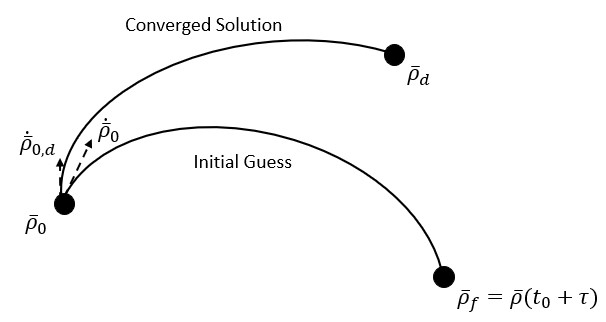
\includegraphics[width=0.75\textwidth]{figures/Targeting.jpg}
    \caption{Simple Targeting Example.}
    \label{fig:targeting}
\end{figure}

The central difference method approximates the slope of the solution at discretized points just
before and after the initial condition:
\begin{equation}
    D\Fbar_{i}(\Xbar_{0})=\frac{\partial\Fbar(\Xbar_{0})}{\partial X_{i}}=\frac{\Fbar(X_{i}+\kappa)-\Fbar(X_{i}-\kappa)}{2\kappa},
    \label{eq:slope}
\end{equation}
where $X_{i}$ is one of the components of the free variable vector and $\kappa$ is a small
perturbation (this investigation selects the square root of the machine tolerance,
$\sqrt{\epsilon}$). Each variable in the free variable vector is perturbed in both directions by
$\kappa$, one at a time, and the constraint vector is evaluated at each new free variable vector
and substituted into \cref{eq:slope} above. Perturbing all of the free variables individually makes
up the numerical Jacobian:
\begin{equation}
    DF(\Xbar_{0})=\begin{bmatrix}   D\Fbar_{1}(\Xbar_{0})   &   \dots   &   D\Fbar_{m}(\Xbar_{0})\end{bmatrix}.
    \label{eq:centraldifference}
\end{equation}
These numerical $DF$ matrices can be compared to their analytical counterparts (such as the example
Jacobian in \cref{eq:exJacobian}) to verify partial derivatives or applied in isolation when
analytical partial derivatives are either not available or exceedingly complex.
